\documentclass[11pt,a4paper,titlepage]{article}
\usepackage[left=2cm,text={17cm,24cm},top=3cm]{geometry}
\usepackage[T1]{fontenc}
\usepackage[czech]{babel}
\usepackage[utf8]{inputenc}

\usepackage{graphicx}

\usepackage{hyperref} % url

\bibliographystyle{czplain}

%uvozovky
\newcommand{\ceskeuvozovky}[1]{\quotedblbase#1\textquotedblleft}
\begin{document}

\begin{titlepage}
\begin{center}
    {\LARGE\textsc{Vysoké učení technické v~Brně}}\\
    \smallskip
    {\Large\textsc{Fakulta informačních technologií}}\\
    \bigskip
    \vspace{\stretch{0.382}}
    \LARGE{Modelování a simulace - projekt}\\
    \smallskip
    \Huge{Produkce řepky v ČR}\\
    \vspace{\stretch{0.618}}
\end{center}
    {\Large Petr Kapoun - xkapou04 \\ Erik Kelemen - xkelem01 \hfill \today }
\end{titlepage}

\tableofcontents
\newpage


\section{Úvod}
I like IMS. I want A. I not nice when not A. I kill garant when not A. Give A.



\section{Postřiky}
Zvolili jsme kompletní řešení postřiků od fitmy BASF\footnote{BASF je německá agrochemická firma, která patří k 
největším na světě.\\https://www.agro.basf.cz/agroportal/cz/cs/startpage.html.}.
Pro určení přibližné ceny jednotlivých postřikových přípravků použijeme ceny existujícího eshopu obchod.agrokop.cz\footnote{AGROKOP CZ, a.s. Třebíč}.
\begin{figure}[ht!]
\centering
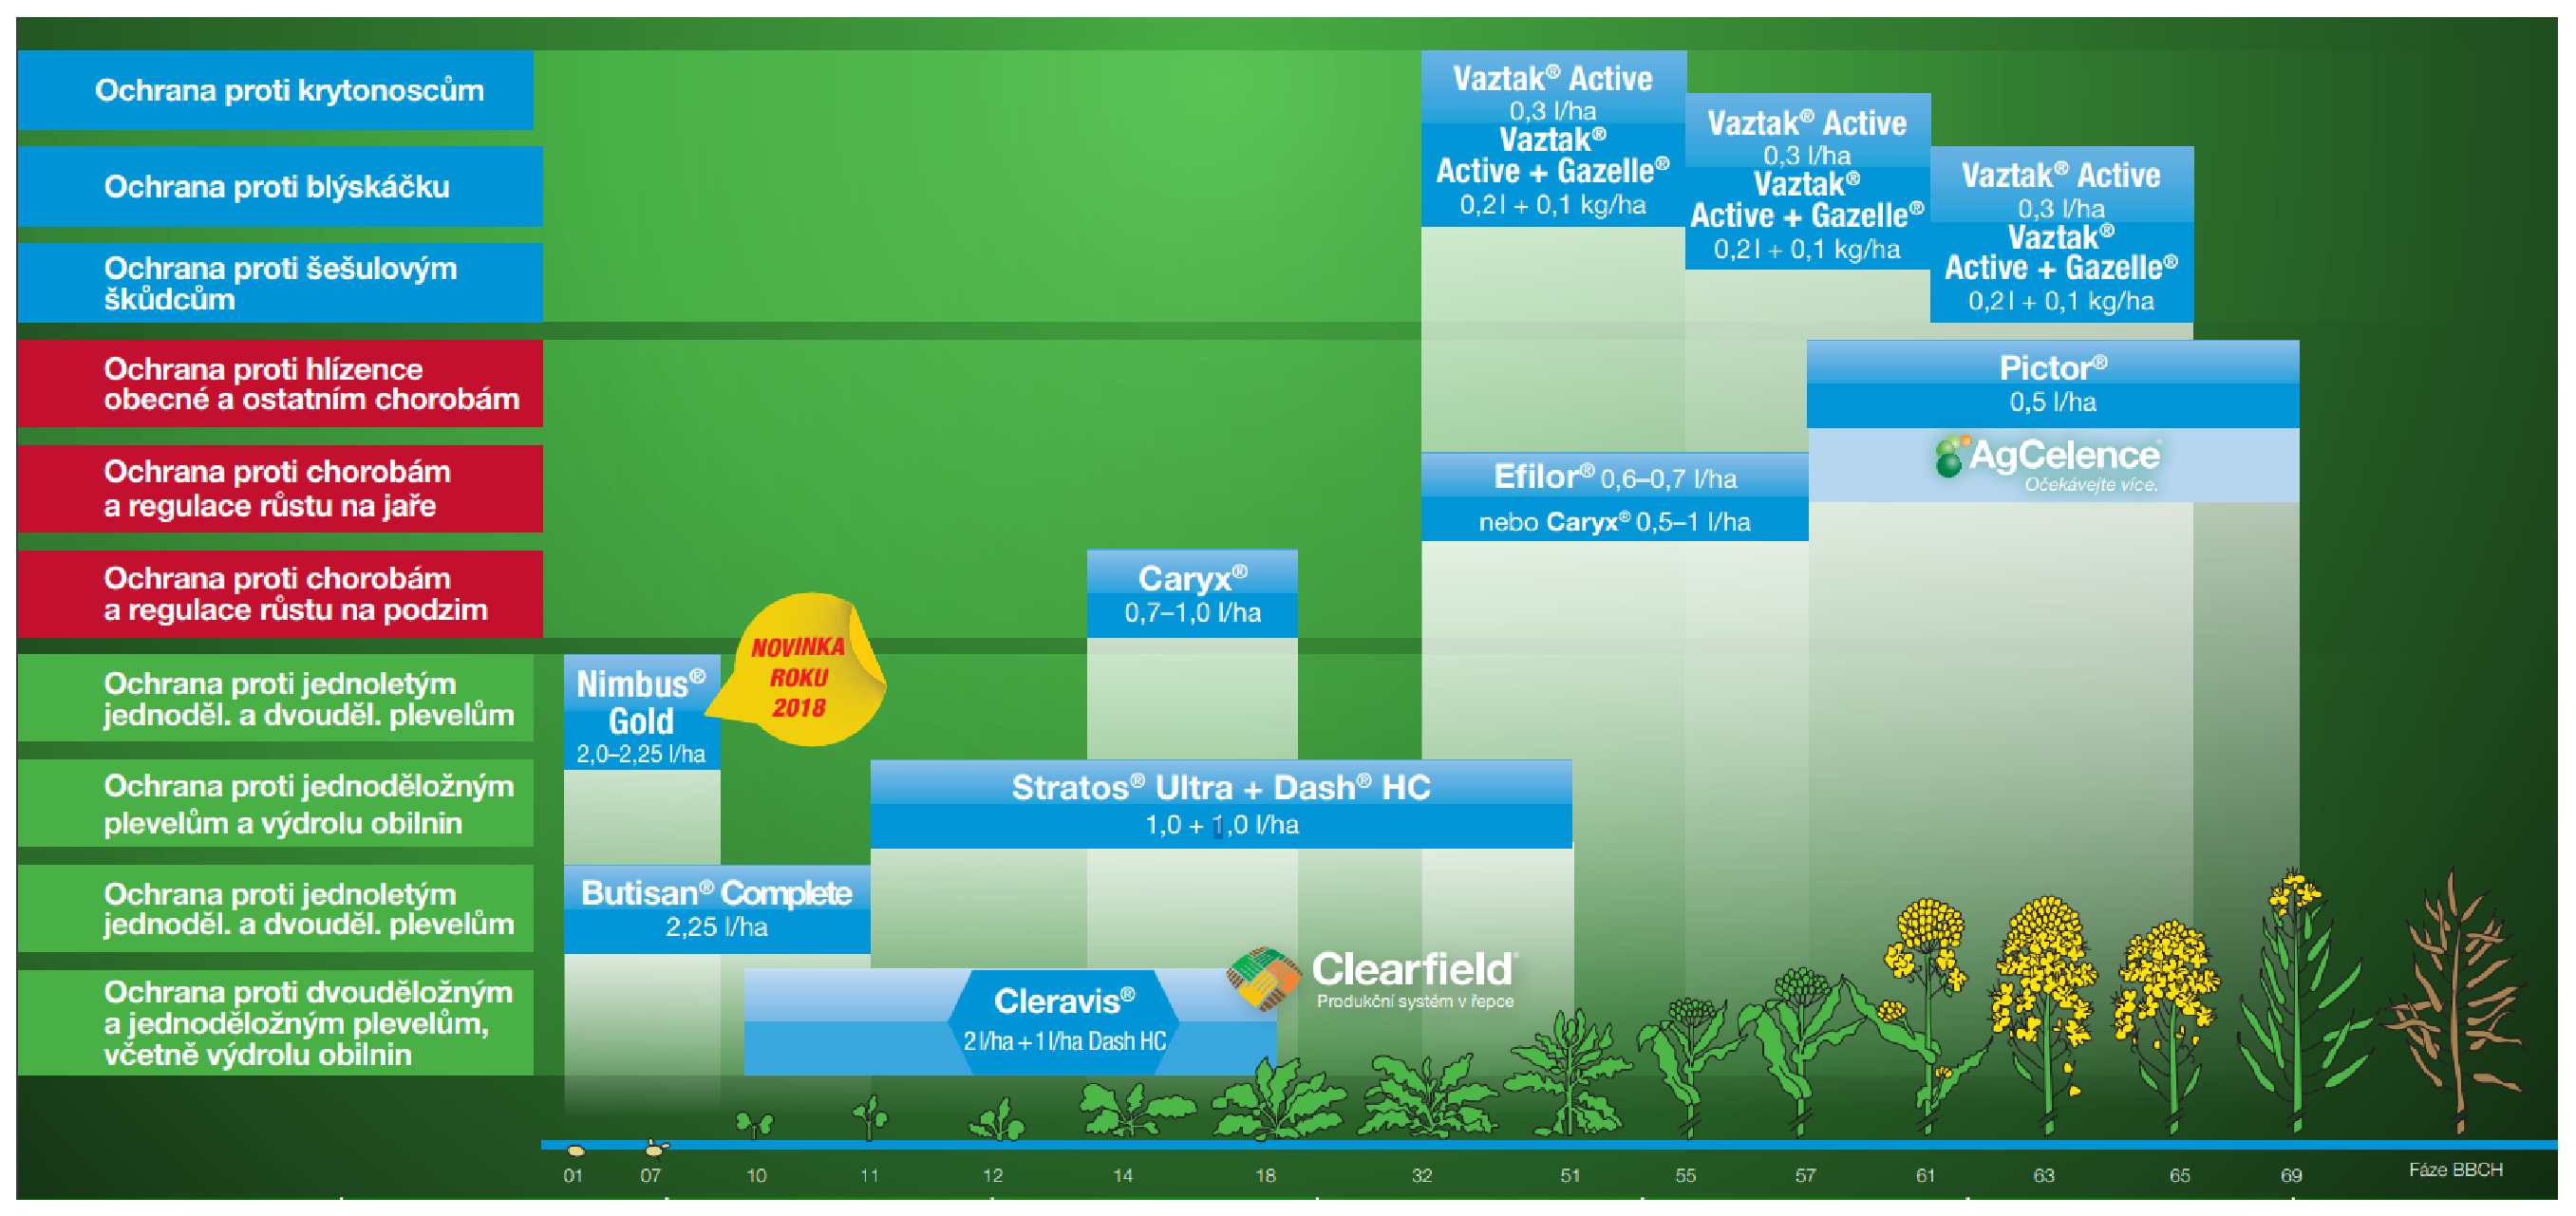
\includegraphics[width=170mm]{img/basf_postriky.eps}
\caption{Ochrana řepky proti škodlivým činitelům firmy BASF \label{basf_postriky}}
\end{figure}
Používané přípravky se dělí do několika skupin, to je důležité hlavně kvůli informaci o mísitelnosti jednotlivých přípravků.
\begin{itemize}
  \item Listová hnojiva.
  \item Fungicidy.
  \item Insekticidy.
  \item Herbicidy.
  \item Graminicidy.
\end{itemize}

\subsection{Ochrana proti krytonoscům, blýskáčku a šešulovým škůdcům}
Použitý přípravek se nazývá Vaztak Active\footnote{Vaztak je přípravek německého výrobce BASF: \\\url{\detokenize{
https://www.agro.basf.cz/agroportal/cz/cs/crop_protection/vyhled_v_n__p__pravk__podle_parametr_/product_details_24923.html
}}
\\\url{\detokenize{
https://www.agro.basf.cz/agroportal/cz/media/migrated/product_files/charakteristiky/CH_Vaztak_Active.pdf}}.}.
Vaztak Active je vysoce účinný světlostabilní pyrethroidní insekticid, určený proti 
některým  druhům  žravého  a  savého  hmyzu,  jeho  larvám  a  vajíčkům.  Účinkuje  
jako dotykový a požerový jed. Není systémovým přípravkem a je proto třeba do statečného množství vody k zabezpečení dobrého krycího postřiku. Přípravek je 
stabilní vůči světlu a má nízkou rozpustnost ve vodě, proto má dobrý reziduální 
účinek na povrchu listů. Povlak Vaztaku Active je odolný vůči dešti za předpokladu, že postřik zaschne dříve, než začne pršet.

\begin{itemize}
  \item Spotřeba 0,3l/ha. * 3 za každé období postřiku.
  \item Doporučené množství vody 200–600 l/ha (polní plodiny, zelenina), 200–1000 l/ha (prostorové plodiny) 
  \item Kategorie Insekticidy.
  \item Mísit lze se vším.
  \item Cena 815 bez DPH za litr.
\end{itemize}

\subsubsection{Aplikace postřiku}

Lze konstatovat, že aplikace proti krytonosci řepkovému je v vhodná po 9 až 11 dní po prvním vrcholu náletu do porostu, u krytonosce čtyřzubého obvykle o 7 až 14 dní později. Předčasné aplikace jsou neúčinné, protože likvidujeme pouze nálety samců a samice nepostihujeme. Proto je vhodné pred postřikem se presvedčit, zda je hektár dostatečne infikován než použijeme postřik.

\subsection{Ochrana proti hlízence obecné a ostatním chorobám}
Použitý přípravek se nazývá Pictor\footnote{Pictor je přípravek německého výrobce BASF: \\\url{\detokenize{
https://www.agro.basf.cz/agroportal/cz/cs/crop_protection/vyhled_v_n__p__pravk__podle_parametr_/product_details_1396.html
}}
\\\url{\detokenize{https://www.agro.basf.cz/agroportal/cz/media/migrated/information_material/brochures_products_1/brochures_products/2014/Pictor_Errata.pdf}}
.}.
Vysokou preventivní a kurativní účinnost zajištuje vyvážený poměr dvou kompatibilních látek - boscalidu a dimoxystrobinu, které působí na dýchací procesy houbových organizmů.
\begin{itemize}
  \item Spotřeba 0,5l/ha.
  \item Doporučené množství vody 200-400l/ha.
  \item Kategorie Fungicidy.
  \item Mísit lze se vším.
  \item Cena 3280 bez DPH za litr.
  \item Hlízenka obecná může způsobit výnosové 
ztráty až 30 \%
\end{itemize}

\subsubsection{Aplikace postřiku}
Postřik je ochranný, preventivní. Aplikuje se jednou. Pro úspěšné použití fungicidů proti hlí-
zence obecné bylo vždy nutné směřovat aplikaci do doby plného květu. 
Oproti stávajícím fungicidům se Pictor vyznačuje vyšší flexibilitou použití. Díky dlouhodobému působení účinných látek je
možné použít Pictor již v době krátce před květem až do konce kvetení.


\subsection{Ochrana proti chorobám a regulace růstu na jaře}
Použitý přípravek se nazývá Efilor\footnote{Efilor je přípravek německého výrobce BASF: \\\url{\detokenize{
https://www.agro.basf.cz/agroportal/cz/cs/crop_protection/vyhled_v_n__p__pravk__podle_parametr_/product_details_72192.html
}}.}.
Efilor zajišťuje vynikající ochranu proti houbovým chorobám a kompaktní porosty s ideální architekturou, které díky tomu rovnoměrně kvetou a dozrávají.
\begin{itemize}
  \item Spotřeba 0,6l/ha.
  \item Doporučené množství vody 150-400l/ha.
  \item Kategorie Fungicidy.
  \item Mísit nelze pouze pýrohubné dávky u Graminicidů.
  \item Cena 1399 bez DPH za litr.
\end{itemize}

\subsubsection{Aplikace postřiku}
Preventivně nebo co nejdříve na počátku výskytu choroby.

\subsection{Ochrana proti chorobám a regulace růstu na podzim}
Použitý přípravek se nazývá Caryx\footnote{Caryx je přípravek německého výrobce BASF: \\\url{\detokenize{
https://www.agro.basf.cz/agroportal/cz/cs/crop_protection/vyhled_v_n__p__pravk__podle_parametr_/product_details_1446.html
}}
\\\url{\detokenize{
https://www.agro.basf.cz/agroportal/cz/media/migrated/information_material/brochures_products_1/brochures_products/2014/Caryx_Errata.pdf
}}.}.
Pouze  homogenní  porost  řepky na jaře na začátku prodlužovacího růstu rostlin umožňuje vytvoření  ideální  architektury  porostu 
později v sezóně a tím rovnoměrného kvetení a tvorby šešulí. 
Rovnoměrný  vývoj,  trvalé  zkrácení  a  zesílení  stonků  a  z  toho 
vyplývající odolnost k poléhání – to jsou vynikající výsledky, které přináší použití přípravku Caryx. 
Výsledkem je vyšší hmotnost tisíce semen. Stejnoměrné dozrávání zvyšuje i kvalitu výnosu a snižuje vlhkost sklízených semen.
\begin{itemize}
  \item Spotřeba 0,75-1l/ha.
  \item Doporučené množství vody 150-400l/ha.
  \item Kategorie Fungicidy.
  \item Mísit nelze pouze pýrohubné dávky u Graminicidů.
  \item Cena 1009 bez DPH za litr.
\end{itemize}

\subsection{Ochrana proti jednoletým jednoděl. a dvouděl. plevelům}
První možný přípravek se nazývá Butisan Complete\footnote{Butisan Complete je přípravek německého výrobce BASF: \\\url{\detokenize{
https://www.agro.basf.cz/agroportal/cz/cs/crop_protection/vyhled_v_n__p__pravk__podle_parametr_/product_details_85632.html
}}.}.
\begin{itemize}
  \item Spotřeba 2-2,25l/ha.
  \item Doporučené množství vody 100-400l/ha.
  \item Kategorie Herbicidy.
  \item Mísit lze se vším.
  \item Cena 1016 bez DPH za litr.
\end{itemize}

\subsection{Ochrana proti jednoděložným plevelům a výdrolu obilnin}
Použitý přípravek se nazývá Stratos Ultra\footnote{Stratos Ultra je přípravek německého výrobce BASF: \\\url{\detokenize{
https://www.agro.basf.cz/agroportal/cz/cs/crop_protection/vyhled_v_n__p__pravk__podle_parametr_/product_details_1429.html
}}
\\\url{\detokenize{
https://www.agro.basf.cz/agroportal/cz/media/migrated/product_files/charakteristiky/CH_Stratos_Ultra.pdf
}}.}.
Stratos  Ultra  je  selektivní  systémový  herbicid,  jehož  účinná  látka  je  přijímána  
zelenými nadzemními částmi rostlin. Účinnost je proto zaručena i v suchých letech,  kdy  mohou  půdní  herbicidy  selhávat.  V  době  ošetření  mají  být  plevelné  
rostliny v plném růstu a vyvinuty tak, aby měly dostatek zelené hmoty pro přijetí 
potřebného množství účinné látky. Účinnost se projeví již za 3–4 dny po ošetření.
\begin{itemize}
  \item Spotřeba 1l/ha.
  \item Doporučené množství vody 200-300l/ha.
  \item Kategorie Herbicidy.
  \item Mísit nelze s listovým hnojivem Solubor.
\end{itemize}
Pomocný přípravek se nazývá Dash HC\footnote{Dash HC je přípravek německého výrobce BASF: \\\url{\detokenize{
https://www.agro.basf.cz/agroportal/cz/cs/crop_protection/vyhled_v_n__p__pravk__podle_parametr_/product_details_1441.html
}}.}.
\begin{itemize}
  \item Spotřeba 1l/ha.
  \item Doporučené množství vody 300l/ha.
\end{itemize}
Cena za 10l přípravku Stratos Ultra a 10l přípravku Dash HC je 6990 bez DPH.

\subsubsection{Aplikace postřiku}
Stratos Ultra se používá v ošetřovaných plodinách po vzejití lipnicovitých plevelů. Termín ošetření se řídí především růstovou fází plevelů, méně už růstovou fází 
kulturní plodiny. Teplé a vlhké počasí nebo příznivé růstové podmínky účinnost 
urychlují, sucho a nízké teploty ji naopak zpomalují. V oblastech s vysokou světelnou intenzitou je vhodnější ošetřovat v podvečerní době.


\subsection{Ochrana proti dvouděložným a jednoděložnám plevelům, včetně výdrolu obilnin}
Použitý přípravek se nazývá Cleravis\footnote{Cleravis je přípravek německého výrobce BASF: \\\url{\detokenize{
https://www.agro.basf.cz/agroportal/cz/cs/crop_protection/vyhled_v_n__p__pravk__podle_parametr_/product_details_55941.html
}}
\\\url{\detokenize{
https://www.agro.basf.cz/agroportal/cz/media/migrated/product_files/charakteristiky/CH_Cleravis.pdf
}}.}.
Selektivní postřikový herbicid ve formě tekutého suspenzního koncentrátu (SC)
k hubení jednoletých dvouděložných a jednoděložných plevelů včetně výdrolu 
obilnin v porostech řepky
\begin{itemize}
  \item Spotřeba 2l/ha.
  \item Doporučené množství vody 300-400l.
  \item Kategorie Herbicidy.
  \item Mísit nelze s Graminicidy.
\end{itemize}
Pomocný přípravek se nazývá Dash HC.
\begin{itemize}
  \item Spotřeba 1l/ha.
  \item Doporučené množství vody 300l/ha.
\end{itemize}
Cena za 10l přípravku Cleravis a 5l přípravku Dash HC je 11699 bez DPH.

\subsubsection{Aplikace postřiku}
Správný termín aplikace Cleravisu je obecně 
dán stádiem plevelů, ve kterém jsou citlivé k herbicidům, méně již růstovou fází 
řepky.
Maximální počet aplikací je 1x v plodině za vegetaci.




\section{Hnojiva}
Zvolili jsme kompletní řešení postřiků od fitmy Timac AGRO\footnote{BASF je německá agrochemická firma, která patří k 
největším na světě.\\https://www.agro.basf.cz/agroportal/cz/cs/startpage.html.}.
\footnote{TIMAC AGRO je průmyslovou společností specializující se na pěstování půdy, výživu rostlin a zvířat.\\\url{\detokenize{
https://www.cz.timacagro.com/rostlinna-vyroba/plodinova-doporuceni/repka-olejka.htmll
}}.}.
Pro určení přibližné ceny jednotlivých postřikových přípravků použijeme ceny existujícího polského eshopu https://www.kupnawozy.pl a také
rakouského espohu https://www.samen-schwarzenberger.at. Z obrázku je patrné, že je možné si vybrat z některých produkrů, tedy není nutné použít všechny.
Proto jsme z nich vybrali jen některé. Informace o konkrétních hnojivech jsme vyčetli z oficiálních etiket produktů,
 které je možné nalézt na stránce eagri.cz
\footnote{Vyhledavač:\\\url{\detokenize{
http://eagri.cz/public/app/rhpub/hnojivaVerejnostQF.do
}}. Příklad etikety:\\\url{\detokenize{
http://eagri.cz/public/app/rhpub/etikety/etiketa_36439.pdf?id=36439
}}.}.
\begin{figure}[ht!]
\centering
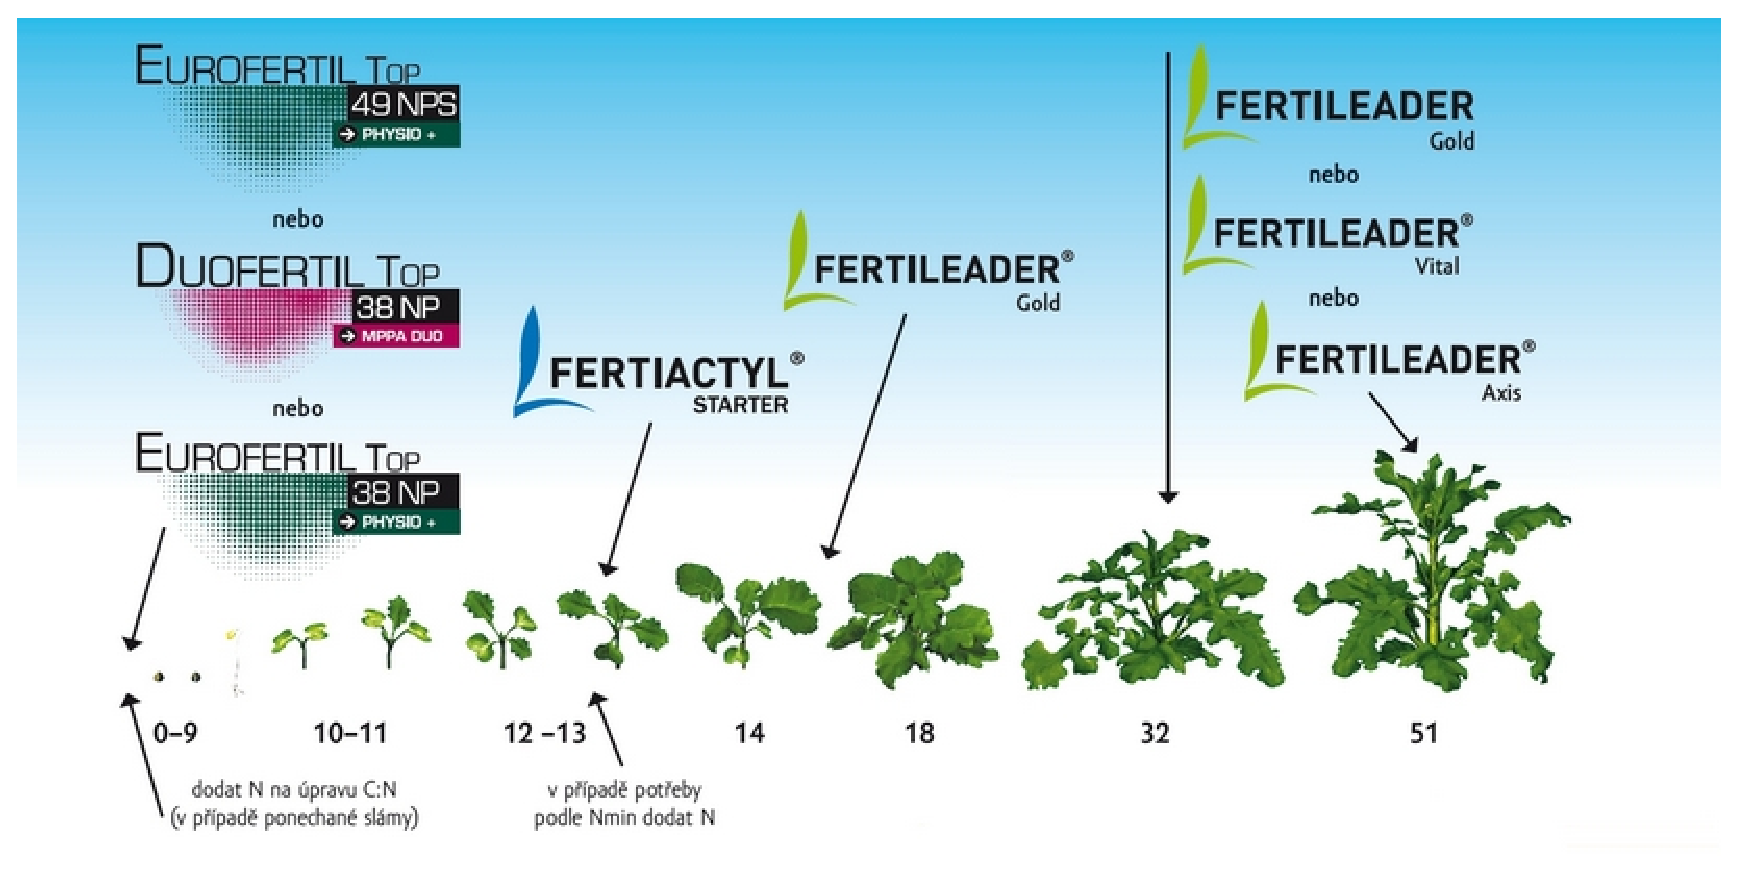
\includegraphics[width=170mm]{img/timac_hnojiva.eps}
\caption{Systém výživy a hnojení řepky ozimé firmy Timac AGRO \label{timac_hnojiva}}
\end{figure}

\subsection{EUROFERTIL TOP 49 NPS}
Obsah látek: (NP 3/22; 24 SO3; 0,15 B; Mescal 975 (29 CaO); Physio+).
\begin{itemize}
  \item Spotřeba 150-250kg/ha.
  \item Cena 2425,0 PLN/t.
\end{itemize}

\subsection{Fertiactyl Starter}
Obsah látek: (13 \% N; 5 \% P2O5; 8 \% K2O; FERTIACTYL® komplex).
\begin{itemize}
  \item Spotřeba kg/ha.
  \item Spotřeba 3l/ha.
  \item Doporučené množství vody 150-500l/ha.
  \item Cena 62,4 PLN/l.
\end{itemize}

\subsection{Fertileader Gold}
Obsah látek: (5,7\%B + 0,35\%Mo + Seactiv).
\begin{itemize}
  \item Spotřeba 3l/ha.
  \item Doporučené množství vody 150-500l/ha.
  \item Cena 16,52 EUR/l.
\end{itemize}

\subsection{Fertileader Vital}
Obsah látek: (9\%N + 5\%P2O5 + 4\%K2O + 0,1\%Mn + 0,05\%B + 0,02\%Cu + 0,02\%Fe + 0,05\%Zn + 0,01\%Mo + Seactiv).
\begin{itemize}
  \item Spotřeba 4l/ha.
  \item Doporučené množství vody 150-500l/ha.
  \item Cena 15,99 EUR/l.
\end{itemize}



\section{Voda}
Při simulaci se sleduje statistika použití vody.



\section{Zemědělské stroje}

\subsection{Traktor a jeho závěsná zařízení}
Výhodou traktoru je jeho univerzálnost. Zvolili jsme traktor John Deere 6210R\footnote{Test traktoru John Deere 6210R: \\\url{\detokenize{
https://www.fwi.co.uk/machinery/mid-range-tractor-test-john-deere-6210r
}},
\\\url{\detokenize{
http://www.danhel.cz/fotogalerie/predvadeci-john-deere-6210r-s-directdrive.html
}}.}.
\begin{itemize}
  \item Spotřeba 37,1 litrů/h.
  \item Dopravní rychlost 13,8-42 km/h.
\end{itemize}

\subsubsection{Secí stroj}
Zvolili jsme secí stroj AMAZONE CAYENA, který si sám kypří půdu\footnote{Technické údaje o stroji AMAZONE CAYENA: \\\url{\detokenize{
https://www.zavesnatechnika.cz/seci-stroj-cayena
}}.}.
\begin{itemize}
  \item Pracovní rychlost 8-15 km/h.
  \item Pracovní záběr 6 m.
\end{itemize}

\subsubsection{Postřikový stroj}
Zvolili jsme nesené postřikovače AMAZONE UF s čelní nádrží FT\footnote{Technické údaje o stroji AMAZONE UF: \\\url{\detokenize{
https://www.zavesnatechnika.cz/obrazky-soubory/uf-a958a.pdf?redir
}}.}.
\begin{itemize}
  \item Pracovní rychlost 10 km/h.
  \item Pracovní záběr 12-30 m.
\end{itemize}

\subsubsection{Rozmetadlo minerálních hnojiv}
Zvolili jsme stroj AMAZONE ZA-M Ultra Profis Hydro\footnote{Technické údaje o stroji AMAZONE ZA-M: \\\url{\detokenize{
https://www.zavesnatechnika.cz/obrazky-soubory/prospekt_amazone_zam-55bc0.pdf?redir
}}.}.
\begin{itemize}
  \item Pracovní rychlost 12 km/h.
  \item Pracovní šířka 30 m.
  \item Pracovní rychlost 27 ha/h.
\end{itemize}

\subsubsection{Rozmetadlo minerálních hnojiv}
Zvolili jsme návěs T730/3\footnote{Technické údaje - NÁVĚS, 12T, T730/3: \\\url{\detokenize{
http://www.agrotechnika.cz/zemedelska-technika/navesy-12t-t730-3/
}}.}  s nosností 12t.
\begin{itemize}
  \item Objem 15,3 $m^3$.
\end{itemize}

\subsection{Sklízecí mlátička}
Zvolili jsme sklízecí mlátičku New Holland CR10.90\footnote{Technické údaje o sklízecí mlátičce CR10.90: \\\url{\detokenize{
https://www.eagrotec.cz/potvrzeno-zapisem-do-guinessovy-knihy-rekordu-sklizeci-mlaticka-cr10.90-je-nejvykonnejsi-mlatickou-na-svete
}}.}. Mlátička má i zásobník, do něj lze ukládat zrna v dobu sklizně. Odpad zůstává na poli.
Traktor zatím jezdí mezi mlátičkou a skladem, mlátička za jízdy přesypává svůj obsah na vůz za traktorem.
\begin{itemize}
  \item Spotřeba 11,14 litrů/ha.
  \item Rychlost 5,9 km/h.
  \item Rychlost sklizně 10,03 ha/h.
  \item Šířka žacího ústrojí: 6,10-12,5 m.
  \item Objem zásobníku zrna 14500 l.
  \item Rychlost vyprázdnění 142 l/m.
\end{itemize}

\pagebreak
\section{Implementácia}

\subsection{Petriho siete}

\begin{figure}[ht!]
\centering
\includegraphics[scale=0.3]{img/WeekGen.png}
\caption{Transakcia "Working hours" počas pracovnej doby}
\end{figure}

\begin{figure}[ht!]
\centering
\includegraphics[scale=0.3]{img/GenPictorTime.png}
\caption{Transakcia "Time for Pictor" počas potreby postreku touto látkou}
\end{figure}

\begin{figure}[ht!]
\centering
\includegraphics[scale=0.3]{img/GenEfilorTime.png}
\caption{Transakcia "Time for Efilor" počas potreby postreku touto látkou}
\end{figure}

\begin{figure}[ht!]
\centering
\includegraphics[scale=0.3]{img/GenCaryxTime.png}
\caption{Transakcia "Time for Caryx" počas potreby postreku touto látkou}
\end{figure}

\begin{figure}[ht!]
\centering
\includegraphics[scale=0.3]{img/GenButisanCompleteTime.png}
\caption{Transakcia "Time for Butisan Complete" počas potreby postreku touto látkou}
\end{figure}

\begin{figure}[ht!]
\centering
\includegraphics[scale=0.3]{img/GenStratosUltraTime.png}
\caption{Transakcia "Time for Stratos Ultra" počas potreby postreku touto látkou}
\end{figure}

\begin{figure}[ht!]
\centering
\includegraphics[scale=0.3]{img/GenCleravisTime.png}
\caption{Transakcia "Time for Cleravis" počas potreby postreku touto látkou}
\end{figure}

\begin{figure}[ht!]
\centering
\includegraphics[scale=0.3]{img/Infestation.png}
\caption{Priebeh infestácie akoukoľvek chorobou/škodcom}
\end{figure}

\begin{figure}[ht!]
\centering
\includegraphics[scale=0.3]{img/Fertilization.png}
\caption{Priebeh hnojenia akýmkoľvek hnojivom}
\end{figure}

\begin{figure}[ht!]
\centering
\includegraphics[scale=0.25]{img/Growing.png}
\caption{Rast repky}
\end{figure}

\begin{figure}[ht!]
\centering
\includegraphics[scale=0.25]{img/Harvest.png}
\caption{Sklizeň}
\end{figure}


\section{Přínosy a nevýhody produkce řepky v ČR/SR}
Produkce řepky je nepřímo dotována, proto bylo na území našeho státu tolik žlutých polí.
Pěstování řepky ale nečí krajinu, velké množství postřiků hubí menší organismy a kontaminuje podzemní vodu.


\newpage
\bibliography{literatura}

\end{document}
